\subsection{Imbalanced Learning}

In this section we with several imbalance learning techniques in the context of binary classification.
Our goal was to develop a system that is capable of predicting which titles have received any awards (as already seen in \ref{tab:binarized_features}, only about 8\% our training records did).
We figured that a similar system could be useful in a number of contexts, like for recommendation and showcasing purposes or for streaming platforms attempting to decide which titles to license when this information isn't already available (for example for newly released titles).

\subsubsection{Resampling techniques}

We established a performance baseline using a KNN classifier with no resampling techniques.
We then experimented with three over-sampling strategies (Random Over-sampling, SMOTE, ADASYN), two under-sampling strategies (Random Under-sampling and Edited Nearest Neighbors) and a combination of both (SMOTEEN). In all cases we resampled the dataset as to obtain a perfect balance between the positive and the negative class.

For each technique we fine tuned the hyperparameters of the classifier searching for the best F1 score: initially we performed random seach on ks between 1 and 100, with euclidean and manhattan distance, both weighting neighbors and not. Since we noticed generally better performance with weighting of exemplars, we removed unweighted models from the grid search.

We also noticed that for over-sampling methods performance was rapidly decreasing as k  got bigger, so we restricted our grid search to odd ks between 1 and 21. Since performance of under-sampling techniques wasn't degrading so rapidly, we extended the number of neighbors considered for these approaches to odd numbers between 1 and 41, but we noticed that scores were nevertheless plateauing around 10, so we didn't consider it necessary to widen the search beyond that.

We then compared performance of different resampling strategies checking precision, recall and F1 score on 5-fold cross validation (cf \ref{tab:imb_learn_cv_performance}).

\begin{table}
    \footnotesize
    \csvautobooktabular{../results/tables/imb_learn_cv_performance.csv}
    \caption{Results of tested resampling methods on 5-fold cross validation.}
    \label{tab:imb_learn_cv_performance}
\end{table}

Precious insights were also gathered by the inspection of the precision-recall curves (reported in fig \ref{fig:imb_learn_cv_pr}) and average precision.

\begin{figure*}
    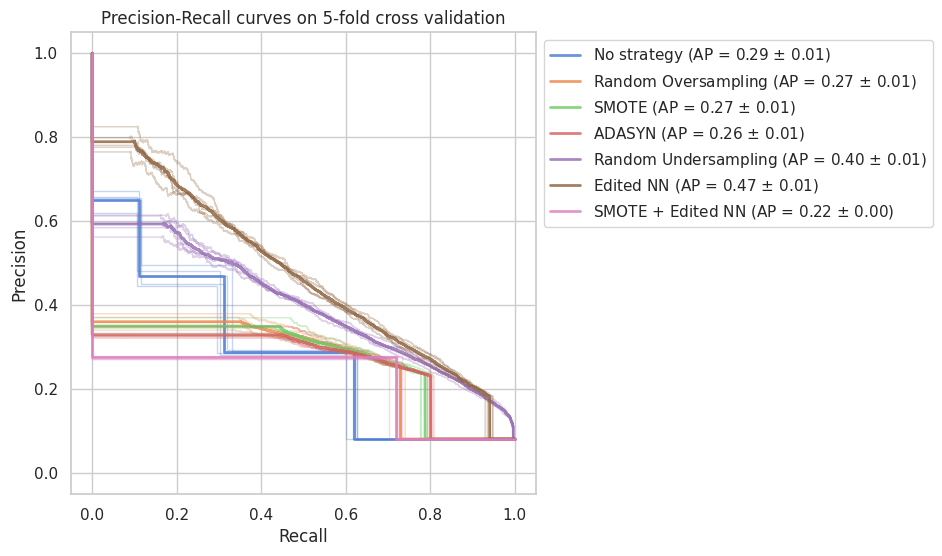
\includegraphics[width=.8\textwidth]{../results/images/imb_learn_cv_pr.png}
    \caption{Precision-Recall curves on 5-fold cross-validation for different resampling methods}
    \label{fig:imb_learn_cv_pr}
\end{figure*}

Over-sampling methods and the combination of SMOTE and Edited NN all show worse ranking capabilities than no resampling strategy at all. In particular these methods demonstrate much worse performance in the early retrieval range of operating points, meaning that they have much more false positives in the top ranked instances.
This is also reflected in the lower precision scores that are not balanced by the higher recall.
In addition to that, over-sampling techniques, even when relatively inexpensive at fitting time (Random Over-sampling), are slower at prediction time (because of the necessity to compute distances with all records in the over-sampled dataset) and have considerably higher space requirements.

Performance obtained with Random Under-sampling has similar F1 score to no resampling strategy, but shows better ranking capabilities, as demonstrated both by AP score and inspection of the PR curve.

The best results are obtained with Edited Nearest Neighbor. The PR curve for ENN almost always dominates random under-sampling with minimal crossing-over for higher values of recall.

It seems to us that Random Under-sampling may be the preferred choice in some context in which fitting time would be a more pressing concern than the precision of the prediction, so we decided to assess both Edited NN and Random Under-sampling on the test set.

\subsubsection{Decision threshold and assessment}
Edited Nearest Neighbor showed satisfactory performance, improving by 0.1 the F1 score of the vanilla KNN and having the best precision among all tested methods (0.50) and recall at least better than the vanilla KNN.
Nevertheless, we decided to post-tune the decision threshold of both our best performing models before assessment on the test set.
For the pipeline using Random Under-sampling this resulted in setting a higher threshold (0.77), while for Edited NN the threshold had to be lowered to 0.38.
Fig \ref{fig:imb_learn_threshold} illustrates the effect of changing the decision threshold for the pipeline using Random Under-sampling: we can observe that at the default threshold the model would have better recall but much worse precision than at the tuned threshold.

\begin{figure}
    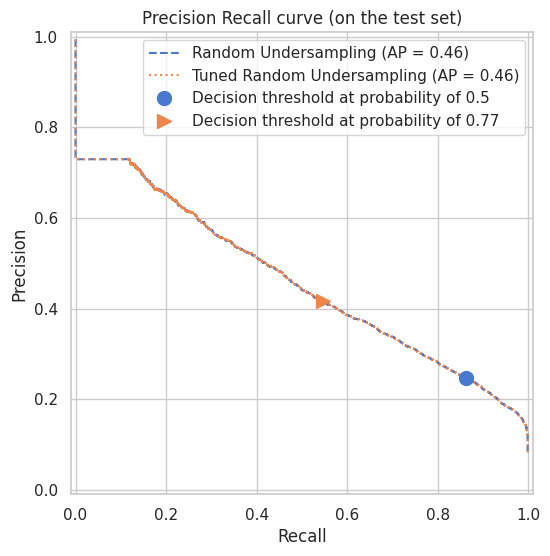
\includegraphics[width=\columnwidth]{../results/images/imb_learn_threshold.png}
    \caption{Decision threshold for KNN with Random Under-sampling before and after tuning.}\label{fig:imb_learn_threshold}
\end{figure}

We finally assessed both models on the test set, obtaining very similar results: ENN obtained a F1 score of 0.49, while Random Under-sampling 0.47; inspecting the other metrics we can confirm that the worse performance of Random Under-sampling is entirely due to a lower precision (0.42 vs 0.44 for ENN), as we had expected from the inspection of the PR curves in validation.
